\chapter{La géométrie de l’espace homogène}

\lectureoverview{La platitude constitue une excellente approximation de l’Univers observé, mais ce n’est pas un principe. Si nous conservons l’homogénéité et l’isotropie tout en autorisant une courbure, trois géométries spatiales simplement connexes se présentent : l’espace euclidien, l’espace sphérique et l’espace hyperbolique. On peut construire leurs métriques à partir de la façon dont les coquilles concentriques grandissent avec la distance, et mettre leur courbure à l’épreuve en mesurant les tailles angulaires et le nombre d’objets. L’espace plat peut aussi être fini si sa topologie est celle d’un tore. Enfin, associer à l’un quelconque de ces espaces homogènes un facteur d’échelle dépendant du temps donne les métriques cosmologiques de l’espace-temps et la loi de Hubble ; la dynamique de ce facteur d’échelle doit découler de la relativité générale.}

\section{La platitude est une observation, pas un principe}

Jusqu’ici, nous avons traité l’espace comme plat et avons presque rien dit de la géométrie de l’espace-temps. Les observations justifient de considérer l’espace comme plat avec une très bonne approximation, mais elles ne font pas de la platitude une loi. Ce que les mesures nous indiquent réellement, c’est que tout rayon de courbure doit être grand devant la région que nous avons cartographiée. L’espace pourrait être exactement plat, courbe positivement ou courbe négativement. Aux échelles très supérieures à la région observable, nous ne savons pas encore laquelle de ces descriptions est correcte.

Nous allons donc relâcher une hypothèse tout en en conservant une autre. Nous ne supposerons pas l’espace plat, mais continuerons à le supposer homogène et isotrope. Il s’agit d’une hypothèse de travail, non d’un article de foi. Pour en étudier les conséquences, nous la posons et effectuons les calculs ; nous pourrons ensuite l’abandonner et nous demander en quoi un Univers inhomogène se comporterait différemment.

L’homogénéité signifie que tous les points ont le même caractère géométrique. Un observateur qui se déplace ailleurs et répète les expériences géométriques locales obtient les mêmes résultats. L’isotropie signifie qu’aucune direction n’est privilégiée. Ces conditions excluent presque toutes les surfaces courbes que l’on dessine spontanément. Un paraboloïde est plus fortement courbé près de son sommet que loin de celui-ci. Un ellipsoïde allongé diffère au niveau de ses pôles et de son ventre. Une sphère bosselée, ou la surface terrestre considérée avec ses montagnes et ses vallées, est courbe mais non homogène. La question cosmologique est plus restreinte :
\begin{quote}
Quels espaces peuvent être courbes tout en présentant la même géométrie depuis chaque point et dans toutes les directions ?
\end{quote}

Si l’on fait abstraction pour le moment des identifications globales, il existe trois réponses à courbure constante : l’espace plat, l’espace sphérique à courbure positive et l’espace hyperbolique à courbure négative. La réserve concernant les identifications globales est importante ; nous construirons plus loin un tore plat fini et corrigerons l’affirmation trop simpliste selon laquelle ces trois géométries épuisent toutes les possibilités.

\section{La métrique et les coordonnées de l’observateur}

Nous commençons par l’espace seul, et non par l’espace-temps. Sa géométrie est encodée dans une métrique : une règle donnant la distance au carré \(ds^2\) entre des points voisins. Une fois cette règle locale connue partout, on peut en déduire les longueurs, les angles, les aires, les volumes, les géodésiques et la courbure.

Dans un plan euclidien et dans l’espace euclidien tridimensionnel, les coordonnées cartésiennes donnent
\begin{equation}
ds_2^2=dx^2+dy^2,
\qquad
ds_3^2=dx^2+dy^2+dz^2.
\label{eq:c03-cartesian-flat}
\end{equation}
L’ajout de la troisième dimension ajoute simplement le terme orthogonal \(dz^2\), mais ce qui importe n’est pas la simplicité de cette formule. C’est que l’équation~\eqref{eq:c03-cartesian-flat} spécifie entièrement la géométrie locale.

\begin{figure}[htbp]
\centering
\includegraphics[width=0.74\textwidth]{lecture_03_figure_02.png}
\caption{La métrique cartésienne de l’espace plat tridimensionnel, telle qu’elle est écrite au tableau.}
\label{fig:c03-cartesian-board}
\lectureframe{00:05:13.138}
\end{figure}

Les coordonnées cartésiennes masquent la façon dont un astronome appréhende l’Univers. Nous occupons un point, regardons au loin dans une certaine direction et classons ce que nous voyons selon l’angle et la distance. Dans un Univers bidimensionnel, le champ visuel formerait littéralement un cercle de directions autour de nous. Les coordonnées polaires ne sont donc pas seulement élégantes : elles mettent en évidence la géométrie angulaire utilisée en cosmologie.

Soit \(r\) la distance radiale et \(\theta\) la direction. Le même plan euclidien a maintenant pour métrique
\begin{equation}
ds^2 = dr^2 + r^2 d\theta^2.
\label{eq:c03-polar-flat}
\end{equation}
Pour un petit angle fixe \(d\theta\), la séparation transverse vaut \(r\,d\theta\). Elle augmente linéairement à mesure que l’on s’éloigne, et sa contribution au carré à la métrique est donc \(r^2d\theta^2\).

Le terme angulaire est lui-même la métrique d’un espace à une dimension. Un cercle est une sphère de dimension un, notée \(S^1\), et la métrique du cercle unité s’écrit conventionnellement
\begin{equation}
d\Omega_1^2 = d\theta^2,
\qquad\text{so that}\qquad
ds^2 = dr^2 + r^2 d\Omega_1^2.
\label{eq:c03-omega-one}
\end{equation}
Le tableau indique \(d\Omega^2\), sans indice lisible ; la définition donnée oralement précise que l’objet visé est \(d\Omega_1^2\).

\begin{figure}[htbp]
\centering
\includegraphics[width=0.74\textwidth]{lecture_03_figure_03.png}
\caption{Le schéma en coordonnées polaires et la métrique de l’espace plat. Le tableau indique \(d\Omega^2\) ; l’explication précise qu’il s’agit de la métrique du cercle unité \(d\Omega_1^2=d\theta^2\).}
\label{fig:c03-polar-board}
\lectureframe{00:08:37.254}
\end{figure}

\begin{figure}[htbp]
\centering
\begin{tikzpicture}[scale=1.2]
\draw[->] (-1.2,0)--(1.8,0);
\draw[->] (0,-1.2)--(0,1.8);
\draw[thick] (0,0)--(1.3,1.1);
\draw (0.7,0.7) node[above] {$r$};
\draw (0.58,0) arc (0:40:0.58);
\draw (0.8,0.22) node {$\theta$};
\end{tikzpicture}
\caption{Reconstitution nette des coordonnées polaires centrées sur l’observateur utilisées dans l’équation~\eqref{eq:c03-omega-one}.}
\label{fig:c03-polar-redraw}
\end{figure}

\begin{classroomqa}
\audiencequestion{Est-ce que \(d\theta^2\) mesure vraiment la distance le long de la circonférence ?}
\lecturerresponse{Oui. Sur un cercle unité, la longueur d’arc est égale à l’angle exprimé en radians ; deux points voisins séparés par \(d\theta\) ont donc une séparation intrinsèque au carré égale à \(d\theta^2\). La circonférence du cercle vaut \(2\pi\), et intégrer \(ds=d\theta\) sur un tour complet donne précisément \(2\pi\). Multiplier par \(r^2\) agrandit le cercle unité jusqu’à obtenir la coquille de rayon \(r\) dans le plan. \lecturetimestamp{00:09:11--00:09:26}}
\end{classroomqa}

Le mot \emph{intrinsèque} est essentiel. Si nous plongeons le cercle unité dans un plan euclidien, nous pouvons le décrire par
\begin{equation}
x^2 + y^2 = 1.
\end{equation}
Cette équation décrit la façon dont le cercle se trouve dans un espace plus vaste. Elle n’est pas nécessaire à un habitant qui ne peut mesurer que les distances le long du cercle. Nous pourrions courber une fibre optique souple pour former une boucle fermée irrégulière, sans l’étirer. Son apparence dans le plan changerait, mais sa circonférence intrinsèque et sa métrique resteraient inchangées. Des incréments égaux de \(\theta\) continueraient à représenter des distances égales le long de la fibre. Il faut donc distinguer la géométrie de la forme contingente que lui confère un plongement.

\begin{figure}[htbp]
\centering
\includegraphics[width=0.64\textwidth]{lecture_03_figure_04.png}
\caption{Le tableau compare un cercle unité rond à une boucle fermée déformée. Si la boucle est courbée sans être étirée, les deux possèdent la même métrique intrinsèque unidimensionnelle.}
\label{fig:c03-intrinsic-board}
\lectureframe{00:10:34.205}
\end{figure}

\begin{figure}[htbp]
\centering
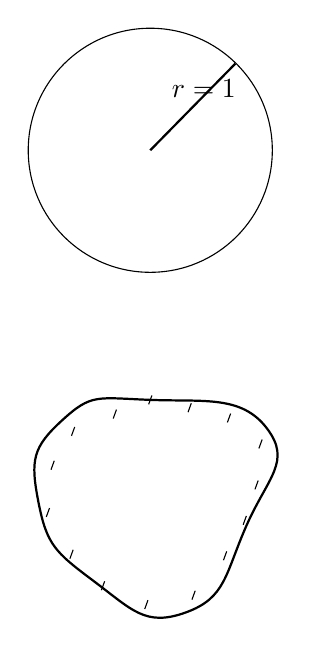
\begin{tikzpicture}[scale=1.0]
\draw (0,0) circle (1.55);
\draw[thick] (0,0)--(1.08,1.1);
\draw (0.68,0.78) node {$r=1$};

\begin{scope}[yshift=-4.35cm]
\draw[thick]
plot[smooth cycle, tension=0.95] coordinates
{(0,1.18) (1.48,0.82) (1.22,-0.42) (0.45,-1.52) (-0.72,-1.12) (-1.42,-0.12) (-1.12,0.92)};
\foreach \p in {(0,1.18),(0.5,1.08),(1.0,0.95),(1.4,0.62),(1.35,0.1),(1.2,-0.35),(0.95,-0.8),(0.55,-1.3),(-0.05,-1.42),(-0.6,-1.18),(-1.0,-0.78),(-1.3,-0.25),(-1.24,0.35),(-0.98,0.78),(-0.45,1.0)}{
\draw[rotate around={70:\p}] \p ++(-0.06,0) -- ++(0.12,0);
}
\end{scope}
\end{tikzpicture}
\caption{La distance intrinsèque subsiste à une déformation extrinsèque : un habitant unidimensionnel mesure la même circonférence dans les deux plongements.}
\label{fig:c03-intrinsic-redraw}
\end{figure}

On peut maintenant interpréter l’espace plat comme une famille emboîtée de cercles centrés sur l’observateur. La coquille située à la distance \(r\) est une copie du cercle unité agrandie d’un facteur \(r\), ce qu’exprime précisément le facteur \(r^2d\Omega_1^2\).

\section{Courbure positive : des coquilles qui se referment}

Une sphère est courbe mais homogène : sur une sphère parfaitement ronde, aucun point ne se distingue géométriquement des autres. Nous pouvons construire sa métrique sans faire appel à une représentation extérieure en trois dimensions. Imaginons des astronomes bidimensionnels vivant sur une sphère unité de dimension \(2\) et plaçant l’origine de leurs coordonnées à l’endroit où ils se trouvent.

Le cercle situé à une petite distance géodésique \(r\) autour d’eux est petit. À mesure que \(r\) augmente, les cercles grandissent, atteignent leur circonférence maximale à mi-parcours autour de la sphère, puis rétrécissent jusqu’à se réduire au point antipodal. Cette croissance et cette contraction se produisent en fonction de la \emph{distance}, et non du temps. La sphère reste statique pendant toute cette construction.

Ici, \(r\) est une distance angulaire le long de la sphère unité, et non une distance euclidienne à partir d’un centre :
\[
0 \le r \le \pi.
\]
L’origine choisie se trouve en \(r=0\), le grand cercle situé à mi-parcours en \(r=\pi/2\), et le point antipodal en \(r=\pi\). Le rayon de la coquille est maintenant \(\sin r\) ; le facteur plat \(r^2\) est donc remplacé par \(\sin^2r\) :
\begin{equation}
d\Omega_2^2 = dr^2 + \sin^2 r\, d\Omega_1^2
            = dr^2 + \sin^2 r\, d\theta^2.
\label{eq:c03-two-sphere}
\end{equation}
Les extrémités et le milieu se comportent exactement comme il faut :
\begin{equation}
\sin 0=0,
\qquad
\sin\frac{\pi}{2}=1,
\qquad
\sin\pi=0.
\end{equation}
Les coquilles partent donc d’une taille nulle, atteignent leur taille maximale, puis se referment.

\begin{figure}[htbp]
\centering
\includegraphics[width=0.82\textwidth]{lecture_03_figure_05.png}
\caption{Passage des cercles emboîtés de l’espace plat aux coquilles sur la sphère. La formule du bas est en partie masquée dans l’image ; la dérivation orale donne le remplacement \(r^2\mapsto\sin^2r\) dans l’équation~\eqref{eq:c03-two-sphere}.}
\label{fig:c03-spherical-board}
\lectureframe{00:16:11.701}
\end{figure}

\begin{figure}[htbp]
\centering
\resizebox{\linewidth}{!}{%
\begin{tikzpicture}[scale=0.92]
\begin{scope}[xshift=-4.15cm]
\draw[->] (-1.7,0)--(1.9,0);
\draw[->] (0,-1.7)--(0,1.9);
\draw (0,0) circle (0.45);
\draw (0,0) circle (0.9);
\draw (0,0) circle (1.35);
\draw[thick] (0,0)--(1.45,1.2);
\draw (0.56,0.18) arc (18:40:0.63);
\draw (0.94,0.44) node {$\theta$};
\end{scope}

\begin{scope}[xshift=4.15cm]
\draw (0,0) circle (2.0);
\fill (0,-2.0) circle (1.5pt);
\fill (2.0,0) circle (1.5pt);
\fill (0,2.0) circle (1.5pt);
\draw[thick] (0,-2.0) arc (-90:90:2.0);
\draw (0,-2.35) node {$r=0$};
\draw (2.75,0) node {$r=\pi/2$};
\draw (0,2.35) node {$r=\pi$};
\end{scope}
\end{tikzpicture}
}%
\caption{Les coquilles plates grandissent indéfiniment, tandis que les coquilles sphériques atteignent leur taille maximale en \(r=\pi/2\) et se referment en \(r=\pi\).}
\label{fig:c03-shells-flat-sphere}
\end{figure}

La notation \(d\Omega_2^2\) désigne la métrique de la sphère unité de dimension \(2\), tout comme \(d\Omega_1^2\) désigne celle de ses coquilles circulaires. La même construction récursive fonctionne une dimension plus haut. À rayon constant dans l’espace plat tridimensionnel, la coquille autour de nous est une sphère de dimension \(2\) :
\begin{equation}
ds_{\text{flat},3}^2 = dr^2 + r^2 d\Omega_2^2.
\label{eq:c03-flat-three-polar}
\end{equation}
Si ces coquilles en sphères de dimension \(2\) grandissent puis se referment selon le facteur \(\sin r\), l’espace obtenu est une sphère unité de dimension \(3\) :
\begin{equation}
d\Omega_3^2 = dr^2 + \sin^2 r\, d\Omega_2^2.
\label{eq:c03-three-sphere}
\end{equation}
La sphère de dimension \(3\) est difficile à se représenter, car son plongement familier nécessiterait quatre dimensions euclidiennes. La métrique, cependant, est complète et ne requiert aucune image. Autour de tout observateur choisi se trouvent des sphères emboîtées de dimension \(2\) ; elles grandissent jusqu’à leur taille maximale, puis rétrécissent jusqu’au point antipodal.

\begin{classroomqa}
\audiencequestion{L’observateur se trouve-t-il au centre de la sphère ?}
\lecturerresponse{L’observateur se trouve au centre des \emph{coquilles de coordonnées}, et non en un centre géométrique privilégié. L’origine est un point de l’espace, et tout autre observateur peut choisir son propre point comme \(r=0\) et obtenir la même métrique. L’homogénéité signifie précisément qu’aucun choix de ce type n’est privilégié. \lecturetimestamp{00:19:21--00:20:27}}
\end{classroomqa}

Pour la seule visualisation, le cercle unité et la sphère unité de dimension \(2\) peuvent être plongés dans des espaces euclidiens :
\begin{equation}
x^2+y^2=1,
\qquad
x^2+y^2+z^2=1.
\end{equation}
Ces équations décrivent des plongements, et non une physique supplémentaire. Une fourmi confinée au cercle ou à la sphère peut déterminer la métrique intrinsèque sans détecter l’espace euclidien environnant. De même, \(S^3\) n’est pas une boule ordinaire dotée d’une mystérieuse frontière. C’est l’espace tridimensionnel complet décrit par l’équation~\eqref{eq:c03-three-sphere}.

\section{Comment la courbure modifie ce que nous observons}

La géométrie devient physique lorsqu’elle modifie une observation. Supposons qu’un objet ait un diamètre transverse connu \(d\), que sa distance radiale \(r\) ait été déduite indépendamment et que son diamètre angulaire \(d\theta\) soit mesuré dans le ciel. Les galaxies fournissent un exemple intuitif approximatif ; la cosmologie de précision utilise des règles étalons et des chandelles étalons calibrées. On peut réunir les informations sur les distances à partir du décalage spectral vers le rouge, de la relation de Hubble, de la luminosité et du calibrage croisé de différentes classes d’objets.

Dans l’espace plat, considérons \(r\) comme constant sur la largeur transverse de l’objet. L’équation~\eqref{eq:c03-polar-flat} donne
\begin{equation}
d^2 = r^2 d\theta^2.
\label{eq:c03-flat-angle-step}
\end{equation}
Par conséquent,
\begin{equation}
d\theta = \frac{d}{r}.
\label{eq:c03-flat-angle}
\end{equation}
La taille angulaire décroît inversement avec la distance.

Sur une sphère unité, la taille transverse de la coquille vaut \(\sin r\) plutôt que \(r\) :
\begin{equation}
d^2 = \sin^2 r\, d\theta^2,
\qquad\text{hence}\qquad
d\theta = \frac{d}{\sin r}.
\label{eq:c03-spherical-angle}
\end{equation}
Pour \(0<r<\pi\), \(\sin r<r\) ; le même objet, à la même distance radiale, paraît donc plus grand que dans l’espace plat. Sa taille angulaire diminue d’abord, atteint un minimum à l’équateur, puis augmente à mesure que la coquille se contracte. Dans l’idéalisation limite au point antipodal, toutes les directions se rejoignent et l’image s’étale sur le ciel.

\begin{classroomqa}
\audiencequestion{Est-ce la même idée que celle utilisée pour déduire la courbure à partir du fond diffus cosmologique ?}
\lecturerresponse{Oui. Le plasma primordial fournit une échelle physique caractéristique par ses oscillations acoustiques. Nous mesurons l’angle sous lequel apparaît cette règle étalon et le comparons à l’angle prévu par chaque géométrie. Les objets n’ont pas besoin d’être littéralement des galaxies ; l’essentiel est de comparer une échelle transverse connue à sa taille angulaire observée. \lecturetimestamp{00:37:37--00:38:12}}
\end{classroomqa}

Le volume des coquilles fournit un second test. En trois dimensions plates, l’aire d’une coquille est proportionnelle à \(r^2\) ; sur une sphère unité de dimension \(3\), elle est proportionnelle à \(\sin^2r\). Une population homogène contient donc d’abord davantage d’objets à mesure que l’on s’éloigne, sur une coquille sphérique, puis moins d’objets après l’équateur. Par rapport à l’espace plat, la courbure positive prédit deux signatures conjuguées : les règles étalons suffisamment éloignées paraissent trop grandes et les coquilles suffisamment lointaines contiennent trop peu d’objets.

\begin{figure}[htbp]
\centering
\resizebox{\linewidth}{!}{%
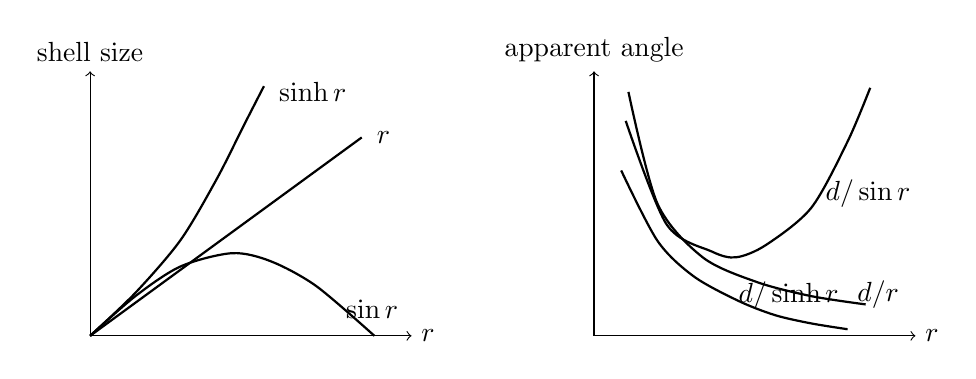
\begin{tikzpicture}[x=1.15cm,y=1.05cm]
\begin{scope}
\draw[->] (0,0)--(3.55,0) node[right] {$r$};
\draw[->] (0,0)--(0,3.2) node[above] {shell size};

\draw[thick] (0,0)--(3.0,2.4);
\draw (3.06,2.4) node[right] {$r$};

\draw[thick]
plot[smooth] coordinates {(0,0) (0.5,0.48) (1.0,0.84) (1.57,1.0) (2.0,0.9) (2.5,0.6) (3.14,0)};
\draw (2.72,0.55) node[below right] {$\sin r$};

\draw[thick]
plot[smooth] coordinates {(0,0) (0.5,0.52) (1.0,1.16) (1.4,1.9) (1.7,2.55) (1.92,3.02)};
\draw (1.98,2.95) node[right] {$\sinh r$};
\end{scope}

\begin{scope}[xshift=6.4cm]
\draw[->] (0,0)--(3.55,0) node[right] {$r$};
\draw[->] (0,0)--(0,3.2) node[above] {apparent angle};

\draw[thick]
plot[smooth] coordinates {(0.38,2.95) (0.7,1.6) (1.2,0.95) (1.8,0.65) (2.4,0.48) (3.0,0.38)};
\draw (2.8,0.5) node[right] {$d/r$};

\draw[thick]
plot[smooth] coordinates {(0.35,2.6) (0.8,1.35) (1.3,1.02) (1.57,0.95) (1.9,1.1) (2.4,1.55) (2.8,2.35) (3.05,3.0)};
\draw (2.45,1.72) node[right] {$d/\sin r$};

\draw[thick]
plot[smooth] coordinates {(0.3,2.0) (0.7,1.15) (1.1,0.72) (1.6,0.42) (2.0,0.25) (2.4,0.15) (2.8,0.08)};
\draw (2.15,0.2) node[above] {$d/\sinh r$};
\end{scope}
\end{tikzpicture}
}%
\caption{Facteurs radiaux des coquilles et lois correspondantes pour la taille angulaire. La courbure positive referme la coquille ; la courbure négative la fait croître exponentiellement.}
\label{fig:c03-shell-angular-laws}
\end{figure}

\begin{classroomqa}
\audiencequestion{La coordonnée radiale devient-elle infinie lorsque nous poursuivons notre chemin autour de la sphère ?}
\lecturerresponse{Non. Sur la sphère unité, \(r\) est une distance angulaire géodésique qui varie uniquement de \(0\) à \(\pi\). En \(r=\pi\), la coquille s’est réduite au point antipodal. Nous étudions ici une géométrie spatiale fixe ; nous ne suivons pas un objet qui s’éloignerait au cours du temps. L’introduction ultérieure d’un rayon de courbure multipliera toutes les distances physiques par ce rayon, sans modifier cet intervalle sans dimension. \lecturetimestamp{00:39:30--00:40:35}}
\end{classroomqa}

\section{La projection n’est pas la géométrie}

Avant de passer à la courbure négative, il est utile de voir à quel point une représentation peut déformer une géométrie pourtant fidèlement décrite. Posons une sphère sur un plan tangent à son pôle Sud. Traçons une droite du pôle Nord passant par chaque point \(P\) de la sphère et prolongeons-la jusqu’au plan en \(P'\). C’est la projection stéréographique. Le pôle Nord lui-même est envoyé à l’infini. Une petite région près du pôle Sud est représentée avec peu de déformation, tandis que des régions intrinsèquement égales près du pôle Nord deviennent énormes sur le plan.

La déformation appartient à la carte, pas à la sphère. La sphère source demeure homogène, même si son image plane attribue des tailles de coordonnées très différentes à des régions équivalentes. Cette distinction nous sera de nouveau nécessaire lorsqu’un espace hyperbolique infini sera comprimé dans un disque fini.

\begin{figure}[htbp]
\centering
\resizebox{\linewidth}{!}{%
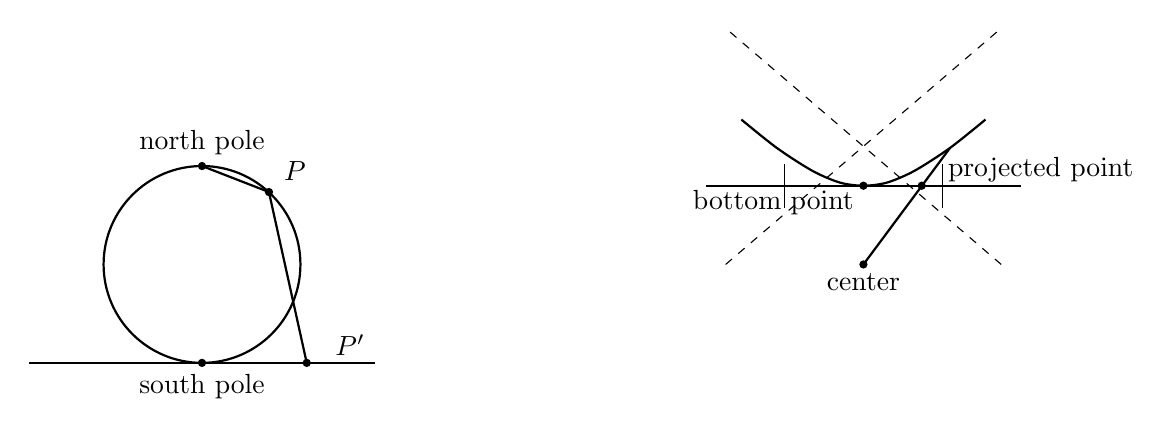
\begin{tikzpicture}[scale=1.0]
\begin{scope}[xshift=-4.2cm]
\draw[thick] (-2.2,-1.25)--(2.2,-1.25);
\draw[thick] (0,0) circle (1.25);
\fill (0,1.25) circle (1.5pt);
\fill (0,-1.25) circle (1.5pt);
\draw (0,1.55) node {north pole};
\draw (0,-1.55) node {south pole};

\fill (0.85,0.92) circle (1.5pt);
\draw (0.92,1.18) node[right] {$P$};
\draw[thick] (0,1.25)--(0.85,0.92)--(1.33,-1.25);
\fill (1.33,-1.25) circle (1.5pt);
\draw (1.57,-1.03) node[right] {$P'$};
\end{scope}

\begin{scope}[xshift=4.2cm]
\draw[thick] (-2.0,1)--(2.0,1);
\draw[dashed] (-1.75,0)--(1.75,3.0);
\draw[dashed] (1.75,0)--(-1.75,3.0);
\draw[thick]
plot[smooth] coordinates
{(-1.55,1.84) (-1.1,1.48) (-0.65,1.19) (-0.3,1.04) (0,1.0) (0.3,1.04) (0.65,1.19) (1.1,1.48) (1.55,1.84)};
\fill (0,0) circle (1.5pt);
\fill (0,1) circle (1.5pt);
\draw (0,-0.22) node {center};
\draw (0,0.78) node[left] {bottom point};
\draw[thick] (0,0)--(1.1,1.48);
\fill (0.74,1.0) circle (1.5pt);
\draw (0.95,1.2) node[right] {projected point};
\draw (-1,0.72) -- (-1,1.28);
\draw (1,0.72) -- (1,1.28);
\end{scope}
\end{tikzpicture}
}%
\caption{À gauche : la projection stéréographique envoie le pôle Nord d’une sphère à l’infini. À droite : un hyperboloïde peut être projeté dans un disque fini, représenté ici par un intervalle en coupe transversale. La déformation des coordonnées ne détruit pas l’homogénéité intrinsèque.}
\label{fig:c03-projections}
\end{figure}

\section{Courbure négative : des coquilles qui grandissent plus vite que dans l’espace plat}

La troisième géométrie homogène simplement connexe remplace \(\sin r\) par le sinus hyperbolique. Ses métriques unitaires en deux et trois dimensions sont
\begin{equation}
dh_2^2 = dr^2 + \sinh^2 r\, d\Omega_1^2,
\label{eq:c03-hyperbolic-two}
\end{equation}
\begin{equation}
dh_3^2 = dr^2 + \sinh^2 r\, d\Omega_2^2.
\label{eq:c03-hyperbolic-three}
\end{equation}
La coordonnée \(r\) varie maintenant sur l’intervalle
\begin{equation}
0\le r<\infty.
\end{equation}
Près de l’origine, \(\sinh r\approx r\), et la géométrie est donc localement euclidienne. Au loin, les coquilles croissent beaucoup plus vite que les coquilles euclidiennes et ne se contractent jamais.

La loi de croissance découle de
\begin{equation}
\sin r = \frac{e^{ir}-e^{-ir}}{2i},
\qquad
\sinh r = \frac{e^r-e^{-r}}{2}.
\label{eq:c03-sin-sinh}
\end{equation}
Pour les grandes valeurs de \(r\), \(\sinh r\sim e^r/2\). En deux dimensions, la circonférence croît donc exponentiellement avec le rayon ; en trois dimensions, l’aire de la coquille croît comme \(\sinh^2r\sim e^{2r}/4\). Une distribution homogène contient en conséquence un très grand nombre d’objets sur une coquille éloignée.

Pour un objet transverse de taille \(d\),
\begin{equation}
d^2 = \sinh^2 r\, d\theta^2,
\qquad\text{so}\qquad
d\theta = \frac{d}{\sinh r}.
\label{eq:c03-hyperbolic-angle}
\end{equation}
Pour les grandes valeurs de \(r\),
\begin{equation}
d\theta \sim 2d\,e^{-r}.
\end{equation}
La courbure négative produit donc une signature opposée à celle de la courbure positive : les règles étalons éloignées paraissent trop petites, tandis que les coquilles éloignées contiennent trop d’objets par rapport à l’espace plat.

\begin{classroomqa}
\audiencequestion{En quoi les domaines de variation radiale distinguent-ils l’espace sphérique de l’espace hyperbolique ?}
\lecturerresponse{Sur la sphère unité, \(r\) s’arrête au point antipodal, \(r=\pi\). Dans l’espace hyperbolique, elle se poursuit sans borne : \(0\le r<\infty\). Le facteur de coquille exprime le même contraste : \(\sin r\) revient à zéro, tandis que \(\sinh r\) croît indéfiniment. \lecturetimestamp{00:52:46--00:53:25}}
\end{classroomqa}

Il existe un plongement qui rend l’homogénéité moins mystérieuse. Introduisons les coordonnées ambiantes \(T,x,y\), où \(T\) est uniquement une coordonnée de plongement et n’est \emph{pas} le temps cosmologique, et prenons la nappe supérieure
\begin{equation}
T^2 - x^2 - y^2 = 1.
\label{eq:c03-hyperboloid}
\end{equation}
Munissons l’espace ambiant de la métrique de signature lorentzienne
\begin{equation}
d\ell_{\mathrm{emb}}^2=-dT^2+dx^2+dy^2.
\label{eq:c03-ambient-minkowski}
\end{equation}
La métrique induite sur l’hyperboloïde est définie positive. Les transformations de Lorentz préservent les deux équations~\eqref{eq:c03-hyperboloid} et~\eqref{eq:c03-ambient-minkowski}, et peuvent déplacer n’importe quel point de la nappe supérieure vers n’importe quel autre. En ce sens, changer l’origine dans l’espace hyperbolique revient à incliner l’axe temporel dans l’espace ambiant auxiliaire. Tous les points sont géométriquement équivalents.

Projeter l’hyperboloïde dans un disque fait s’accumuler les points situés à l’infini sur le cercle frontière. Les régions proches sont représentées presque fidèlement ; celles qui sont plus éloignées sont comprimées de plus en plus fortement. Il s’agit de la représentation sur le disque de Poincar\'e, familière grâce aux figures répétitives d’anges et de démons. Une transformation des coordonnées peut déplacer au centre une figure qui paraît minuscule près du bord, où elle devient grande, tout en préservant toutes les longueurs et tous les angles intrinsèques. En trois dimensions, le modèle correspondant est une boule plutôt qu’un disque. Les noms \emph{Poincar\'e espace}, \emph{espace de Lobatchevski} et \emph{espace à courbure négative constante} désignent cette même géométrie locale.

\begin{classroomqa}
\audiencequestion{Le disque fini est-il comparable à un diagramme de Penrose ?}
\lecturerresponse{La comparaison vaut dans le sens limité où un domaine infini est représenté à l’intérieur d’une figure finie. Ici, toutefois, le disque représente l’espace seul, et non l’espace-temps ou l’infini causal. Sa frontière est à une distance infinie selon la métrique hyperbolique intrinsèque, même si le dessin la place à un rayon de coordonnées fini. \lecturetimestamp{01:02:55--01:03:05}}
\end{classroomqa}

\section{Le rayon de courbure}

Les métriques écrites jusqu’ici décrivent des géométries unitaires. Pour attribuer à l’espace sphérique ou hyperbolique un rayon de courbure arbitraire, multiplions toutes les longueurs par une constante. Le tableau note cette constante \(a\) ; afin d’éviter de la confondre avec le facteur d’échelle cosmologique dépendant du temps que nous utiliserons plus loin, nous noterons le rayon de courbure statique \(R_c\). Comme la métrique mesure le carré des longueurs,
\begin{align}
ds_{\mathrm{sph}}^2
  &=R_c^2d\Omega_n^2
   =R_c^2\left(dr^2+\sin^2r\,d\Omega_{n-1}^2\right),\\
ds_{\mathrm{hyp}}^2
  &=R_c^2dh_n^2
   =R_c^2\left(dr^2+\sinh^2r\,d\Omega_{n-1}^2\right).
\label{eq:c03-scaled-curvature}
\end{align}
La distance radiale physique est \(R_cr\). Augmenter \(R_c\) rend l’espace moins courbe ; la valeur absolue de la courbure sectionnelle constante varie comme \(1/R_c^2\). À la limite \(R_c\to\infty\), les deux métriques courbes tendent vers la géométrie euclidienne dans toute région fixe de taille finie.

\begin{classroomqa}
\audiencequestion{Si l’on double la taille de la sphère, sa courbure augmente-t-elle ou diminue-t-elle ?}
\lecturerresponse{Elle diminue. La première réponse proposée en classe a été corrigée en comparant un ballon de basket à la Terre : sur une distance donnée, la surface plus petite se courbe plus rapidement. Doubler \(R_c\) réduit de moitié l’échelle de courbure proportionnelle à l’inverse du rayon et divise par quatre la courbure sectionnelle \(1/R_c^2\). \lecturetimestamp{01:10:14--01:10:56}}
\end{classroomqa}

Cela explique pourquoi les trois géométries se ressemblent à proximité. Pour \(r\ll1\),
\begin{equation}
\sin r=r-\frac{r^3}{6}+\cdots,
\qquad
\sinh r=r+\frac{r^3}{6}+\cdots.
\end{equation}
Le terme dominant de chacune des deux métriques courbes est la métrique polaire plate ; la courbure apparaît d’abord dans des corrections d’ordre relatif \((L/R_c)^2\) à l’échelle physique \(L\).

\begin{classroomqa}
\audiencequestion{Les observations nous disent-elles si l’espace est plat, sphérique ou hyperbolique ?}
\lecturerresponse{Elles nous disent que la région observable est très proche d’un espace plat. L’estimation grossière donnée en cours était qu’une borne de un pour cent sur les effets de courbure implique \(R_c\) au moins environ dix fois la taille de la région visible, puisque \((L/R_c)^2\lesssim10^{-2}\). Le volume de courbure correspondant serait alors au moins de l’ordre de \(10^3\) volumes visibles. Il s’agit d’une estimation de cours en ordre de grandeur, et non d’une citation de données de précision actuelles ; la platitude exacte reste la possibilité \(R_c=\infty\). \lecturetimestamp{01:11:00--01:13:37}}
\end{classroomqa}

\section{Plat mais fini : le tore}

Nous devons maintenant corriger l’affirmation selon laquelle les espaces plat, sphérique et hyperbolique seraient les seules possibilités homogènes. Ce sont les trois géométries à courbure constante simplement connexes. Un espace plat peut aussi avoir une topologie globale non triviale.

Partons d’un rectangle euclidien. Identifions point par point son côté gauche à son côté droit, et son bord inférieur à son bord supérieur. En franchissant n’importe quel bord, on revient par le bord opposé. La métrique locale reste \(dx^2+dy^2\), mais l’espace global est périodique et fini. Ce quotient est un tore plat bidimensionnel \(T^2\). Une dimension périodique donne un cercle \(T^1\) ; identifier les faces opposées d’un parallélépipède rectangle donne un tore plat tridimensionnel \(T^3\), et la construction s’étend à un nombre quelconque de dimensions.

\begin{figure}[htbp]
\centering
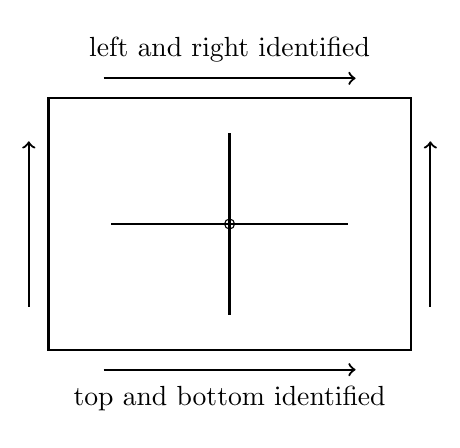
\begin{tikzpicture}[scale=1.0]
\draw[thick] (0,0) rectangle (4.6,3.2);

\draw[->,thick] (0.7,3.45)--(3.9,3.45);
\draw[->,thick] (0.7,-0.25)--(3.9,-0.25);

\draw[->,thick] (-0.25,0.55)--(-0.25,2.65);
\draw[->,thick] (4.85,0.55)--(4.85,2.65);

\draw[thick] (0.8,1.6)--(3.8,1.6);
\draw[thick] (2.3,0.45)--(2.3,2.75);

\draw (2.3,1.6) circle (1.8pt);

\draw (2.3,-0.62) node {top and bottom identified};
\draw (2.3,3.82) node {left and right identified};
\end{tikzpicture}
\caption{Un tore plat construit en identifiant les côtés opposés d’un rectangle. Les côtés ne sont pas des frontières : les points appariés sont un seul et même point de l’espace quotient.}
\label{fig:c03-flat-torus}
\end{figure}

\begin{classroomqa}
\audiencequestion{L’Univers peut-il donc être à la fois plat et fini ?}
\lecturerresponse{Oui. La platitude est une propriété locale de la métrique ; la finitude peut être une propriété globale de la topologie. Un tore tridimensionnel suffisamment grand paraîtrait euclidien dans toute la région que nous pouvons observer, même si son volume total est fini. \lecturetimestamp{01:13:37--01:17:59}}
\end{classroomqa}

La représentation par revêtement universel rend manifeste la conséquence observable. Au lieu d’identifier les bords, pavons un plan euclidien infini avec des copies du rectangle fondamental. Un objet unique dans le tore apparaît une fois dans chaque copie. En trois dimensions, les copies forment un réseau périodique semblable à un cristal.

\begin{classroomqa}
\audiencequestion{Pourrions-nous vivre dans un Univers torique sans nous en apercevoir ?}
\lecturerresponse{Oui, si la cellule fondamentale est plus grande que la région d’où la lumière nous est parvenue. Si elle était suffisamment petite, la lumière pourrait parcourir les identifications et nous verrions des images répétées des mêmes galaxies, voire des vues répétées de notre propre voisinage, dans différentes directions. La géométrie locale resterait plate dans les deux cas. \lecturetimestamp{01:18:16--01:22:04}}
\end{classroomqa}

\begin{classroomqa}
\audiencequestion{Pourquoi la sphère s’arrête-t-elle à son point antipodal alors que le tore se répète ?}
\lecturerresponse{Sur la sphère, la coquille qui nous entoure rétrécit réellement jusqu’à s’annuler en \(r=\pi\) ; toutes les directions radiales se rejoignent au point antipodal. Sur un tore, le bord d’une cellule rectangulaire choisie ne rétrécit jamais. Il est identifié à un bord opposé de même taille, si bien que le franchir prolonge le même espace dans une description en coordonnées périodiques. \lecturetimestamp{01:22:06--01:23:02}}
\end{classroomqa}

\section{De l’espace à l’espace-temps}

Nous pouvons maintenant réintroduire le temps. Dans les unités où la vitesse de la lumière vaut \(c=1\), la métrique de Minkowski est
\begin{equation}
ds^2 = -dt^2 + dx^2 + dy^2 + dz^2.
\label{eq:c03-minkowski}
\end{equation}
La convention de signe est un choix ; l’essentiel est que le terme temporel ait le signe opposé à celui des termes spatiaux. Un rayon lumineux suit une trajectoire nulle,
\begin{equation}
ds^2 = 0.
\end{equation}
Pour un mouvement le long de \(x\) seulement,
\begin{equation}
-dt^2 + dx^2 = 0
\qquad\Rightarrow\qquad
dx = \pm dt.
\label{eq:c03-null-flat}
\end{equation}
Les deux signes décrivent la lumière se déplaçant vers la gauche ou vers la droite à vitesse un.

En cosmologie, conservons le terme de temps propre \(-dt^2\), remplaçons la partie spatiale euclidienne par une métrique spatiale homogène et laissons son facteur d’échelle global varier dans le temps. Nous notons ce facteur d’échelle \(a(t)\). Il s’agit maintenant d’une fonction dynamique plutôt que du rayon fixe \(R_c\) utilisé dans la comparaison statique.

Comme exemple représentable, prenons un espace-temps de dimension \(2+1\) :
\begin{equation}
ds^2 = -dt^2 + a(t)^2 d\Omega_2^2.
\label{eq:c03-two-plus-one}
\end{equation}
À chaque instant fixé \(t\), l’espace est une sphère de dimension \(2\) et de rayon \(a(t)\). Empiler ces sphères au cours du temps donne l’espace-temps. La construction familière en dimension \(3+1\) est
\begin{equation}
ds^2 = -dt^2 + a(t)^2 d\Sigma^2,
\label{eq:c03-frw-general}
\end{equation}
où \(d\Sigma^2\) est une métrique spatiale unitaire indépendante du temps. Les trois cas simplement connexes sont
\begin{align}
\text{flat:}\quad
ds^2&=-dt^2+a(t)^2\left(dx^2+dy^2+dz^2\right),\label{eq:c03-frw-flat}\\
\text{spherical:}\quad
ds^2&=-dt^2+a(t)^2d\Omega_3^2,\label{eq:c03-frw-spherical}\\
\text{hyperbolic:}\quad
ds^2&=-dt^2+a(t)^2dh_3^2.\label{eq:c03-frw-hyperbolic}
\end{align}
Les coordonnées comobiles conservent leurs proportions relatives tandis que \(a(t)\) varie. Dans les normalisations sphérique et hyperbolique, \(a(t)\) est aussi le rayon de courbure instantané. Dans le cas plat, on peut absorber sa normalisation absolue dans les coordonnées comobiles.

La loi de Hubble s’obtient avant même de poser une équation de champ gravitationnel. Considérons deux points comobiles voisins dont la séparation en coordonnées \(\chi\) est fixe. Leur distance physique est
\begin{equation}
D(t)=a(t)\chi.
\label{eq:c03-comoving-distance}
\end{equation}
En dérivant à \(\chi\) constant, on obtient
\begin{equation}
V=\dot D=\dot a(t)\chi.
\end{equation}
En éliminant \(\chi\),
\begin{equation}
V = \frac{\dot a}{a} D.
\label{eq:c03-hubble-law}
\end{equation}
Ainsi,
\begin{equation}
H = \frac{\dot a}{a}.
\label{eq:c03-hubble-parameter}
\end{equation}
C’est une identité cinématique pour l’expansion ou la contraction homogène. Elle vaut pour les trois géométries spatiales : \(\dot a>0\) donne un éloignement, et \(\dot a<0\) une approche.

La géométrie seule ne détermine pas \(a(t)\). Des fonctions telles que
\begin{equation}
a(t)\propto t^{2/3},
\qquad
a(t)\propto t^{1/2},
\qquad
a(t)\propto e^{Ht}
\end{equation}
satisfont toutes l’ansatz de métrique homogène, mais décrivent des contenus différents en matière et en énergie cosmiques. La relativité générale fournit l’équation dynamique qui permet de choisir entre elles. L’équation de Friedmann qui en résulte reliera également les cas plat, sphérique et hyperbolique aux possibilités d’énergie nulle, négative et positive de la cosmologie newtonienne étudiée précédemment.

\begin{classroomqa}
\audiencequestion{La géométrie et l’évolution cosmique pourraient-elles être beaucoup plus complexes que dans ces modèles ?}
\lecturerresponse{Bien sûr. L’homogénéité et l’isotropie sont des hypothèses restrictives, retenues parce qu’elles sont naturelles, concordent avec les observations à grande échelle et se prêtent bien au traitement mathématique. Il existe de nombreuses géométries et évolutions plus complexes. Une question dynamique importante est de savoir si de vastes classes de modèles initialement irréguliers évoluent vers l’une de ces formes homogènes simples. \lecturetimestamp{01:36:00--01:36:50}}
\end{classroomqa}

\begin{classroomqa}
\audiencequestion{La \(3\)-sphère est-elle la frontière d’un objet à quatre dimensions ?}
\lecturerresponse{On peut la représenter ainsi par plongement, mais l’espace cosmologique est la \(3\)-sphère elle-même. Elle possède trois dimensions intrinsèques et n’a pas de frontière. La représentation dans l’espace euclidien à quatre dimensions n’est qu’un artifice facultatif ; l’équation~\eqref{eq:c03-three-sphere} définit déjà entièrement la géométrie. \lecturetimestamp{01:36:55--01:37:59}}
\end{classroomqa}

\begin{classroomqa}
\audiencequestion{La luminosité est-elle le seul moyen d’obtenir la distance nécessaire au test de courbure ?}
\lecturerresponse{Non. Les raies spectrales permettent de déterminer le décalage vers le rouge, les échelles de distance établies à proximité servent à calibrer la relation de Hubble, et les supernovæ fournissent des luminosités approximativement standard. Ces méthodes sont recoupées plutôt que considérées comme fiables isolément. Même la loi de luminosité en inverse du carré dépend de la géométrie, car l’aire d’un front d’onde est déterminée par \(r^2\), \(\sin^2r\) ou \(\sinh^2r\). C’est la concordance de plusieurs observables qui étaye l’hypothèse d’une géométrie presque plate. \lecturetimestamp{01:38:00--01:41:07}}
\end{classroomqa}

\section{À retenir}

La géométrie d’un univers homogène se lit dans la croissance des coquilles autour de tout observateur :
\begin{equation}
f(r)=
\begin{cases}
r, & \text{flat space},\\
\sin r, & \text{positive curvature},\\
\sinh r, & \text{negative curvature}.
\end{cases}
\end{equation}
La métrique spatiale est \(dr^2+f(r)^2d\Omega_{n-1}^2\). La même fonction détermine les tailles angulaires et le nombre d’objets présents sur une coquille ; la courbure a donc une signification observationnelle directe. Un grand rayon de courbure masque localement ces différences, et une identification torique montre que la courbure locale ne détermine pas à elle seule la taille ni la topologie globales.

Ajouter \(-dt^2\) et le facteur commun \(a(t)^2\) transforme chacune des trois métriques spatiales homogènes en un espace-temps cosmologique. On obtient aussitôt \(V=HD\) avec \(H=\dot a/a\), mais \(a(t)\) reste indéterminé. L’étape suivante ne consiste donc pas à poursuivre l’étude de la géométrie. Il faut aborder le problème dynamique : utiliser les équations d’Einstein pour déterminer comment la matière, le rayonnement, la courbure et les autres formes d’énergie font évoluer le facteur d’échelle.
